\documentclass[12pt,a5paper,titlepage, main = russian]{article}
\usepackage[T1,T2A]{fontenc}
\usepackage[utf8]{inputenc}
\usepackage[warn]{mathtext}
\usepackage{textcomp}
\usepackage[russian]{babel}
\usepackage{extsizes}
\usepackage[left = 1 cm, right = 1 cm, top = 1.5 cm, bottom = 1.5 cm]{geometry}
\usepackage [pagestyles, raggedright]{titlesec}
\usepackage{graphicx}
\usepackage{ragged2e}
\usepackage{amsmath}
\usepackage{pgfplots}
\pagestyle{empty}
\usepackage{tikz}
\usetikzlibrary{patterns}

\usepackage{wrapfig}

\usepackage{siunitx} % Required for alignment
\usepackage{multirow}
\usepackage{rotating}
\usepackage{float}
\usepackage{booktabs}

\usepackage{amsmath,amsfonts,amssymb,amsthm,mathtools} % AMS
\usepackage{icomma}
\usepackage[russian]{babel}
\usepackage[T2A]{fontenc}
\usepackage[utf8]{inputenc}
\usepackage{mathtext}
\usepackage{amsfonts}
\usepackage{ amssymb }
\usepackage{amsmath}
\usepackage{graphics}
\usepackage{graphicx}
\usepackage{wrapfig}
\usepackage{geometry}
\usepackage{float}

\usepackage{wrapfig}
\usepackage{graphicx}
\usepackage{mathtext}
\usepackage{amsmath}
\usepackage{siunitx} % Required for alignment
\usepackage{subfigure}
\usepackage{multirow}
\usepackage{rotating}
\usepackage{afterpage}
\usepackage[T1,T2A]{fontenc}
\usepackage[russian]{babel}
\usepackage{caption}
\usepackage[arrowdel]{physics}
\usepackage{booktabs}
\usepackage{float}


\begin{document}

\begin{titlepage}
\begin{center}
    \small{Министерство науки и высшего образования Российской Федерации}\\
    ФЕДЕРАЛЬНОЕ ГОСУДАРСТВЕННОЕ АВТОНОМНОЕ ОБРАЗОВАТЕЛЬНОЕ УЧРЕЖДЕНИЕ ВЫСШЕГО ОБРАЗОВАНИЯ "МОСКОВСКИЙ ФИЗИКО-ТЕХНИЧЕСКИЙ ИНСТИТУТ (НАЦИОНАЛЬНЫЙ ИССЛЕДОВАТЕЛЬСКИЙ УНИВЕРСИТЕТ)"\\
    (МФТИ, Физтех)
\end{center}
\vspace{2.5cm}
{\huge
    \begin{center}
        {\bf Отчёт о выполнении лабораторной работы}\\
        Изучение сверхтонкой структуры спектральных линий
    \end{center}
}
\vspace{1.5cm}
\begin{flushright}
    {\large Авторы:\\  
Кулиш Павел \\
Куценко Екатерина \\
        \vspace{0.2cm}
        
        Б03-303}
\end{flushright}
\vspace{0.3cm}
\begin{center}
        Москва, \\
        Долгопрудный, 2026 г
\end{center}

\end{titlepage}


\tableofcontents
\newpage



\section{Цель работы}
\begin{itemize}
    \item Регистрация сверхтонкой структуры сперктральных линий.
    \item Изучение методики работы со сканирующим интерферометром Фабри-Перо.
\end{itemize}
\section{Теоретическая сводка}
\subsection{Энергетические уровни и переходы} 
Атом обладает дискретными уровнями энергии. При переходе электрона между уровнями \(E_i\) и \(E_k\) излучается или поглощается фотон, частота которого определяется разностью энергий этих уровней (условие Бора):\\
    \begin{equation}
        h\nu_{ik} = E_i - E_k
    \end{equation}
\\
\subsubsection{Моменты атома (квантование)} 
Состояние электрона в атоме описывается набором квантовых чисел. Полный орбитальный момент \(L\), полный спиновый момент \(S\) и полный момент \(J\) (сумма орбитального и спинового) квантуются, т.е. их абсолютные значения могут принимать только строго определённые величины.

    \begin{equation}
        |L| = \frac{h}{2\pi}\sqrt{L(L+1)}
    \end{equation}
    \begin{equation}
        |S| = \frac{h}{2\pi}\sqrt{S(S+1)}
    \end{equation}
    \begin{equation}
        |J| = \frac{h}{2\pi}\sqrt{J(J+1)}
    \end{equation}      
\subsubsection{Правила отбора} \\
Не все переходы между уровнями разрешены. Существуют правила отбора, определяющие, какие изменения квантовых чисел возможны при излучении или поглощении фотона.

\begin{equation}
    \Delta L = \pm 1,\quad \Delta S = 0 
\end{equation}


\subsection{Типы расщепления спектральных линий} 
Спектральные линии на самом деле имеют сложную структуру и могут состоять из нескольких близкорасположенных компонент. Это связано с несколькими физическими механизмами.

\begin{enumerate}
    \item \textit{Тонкая структура (мультиплетность):} возникает из-за спин-орбитального взаимодействия. Уровень с заданными \(L\) и \(S\) расщепляется на несколько подуровней с разными \(J\). Число компонент = \(2S+1\) (если \(L > S\)) или \(2L+1\) (если \(L < S\)).
    \item \textit{Изотопическое смещение:} вызвано различием масс ядер у разных изотопов одного элемента, что приводит к небольшому сдвигу их спектральных линий друг относительно друга.
    \item \textit{Сверхтонкая структура (СТС):} обусловлена взаимодействием электронной оболочки с ядром атома (его магнитным и механическим моментами). Это расщепление значительно меньше тонкого.
\end{enumerate}

\subsection{Характеристики ядра и СТС} 
Атомное ядро обладает собственным механическим моментом (спином) \(I\) и связанным с ним магнитным моментом. Взаимодействие магнитного момента ядра с магнитным полем, создаваемым электронной оболочкой, приводит к дополнительному расщеплению энергетических уровней.\\
Спин ядра \(I\) квантуется аналогично электронным моментам:
\begin{equation}
    \ |\vec{I}| = \frac{h}{2\pi}\sqrt{I(I+1)} 
\end{equation}


\subsubsection{Полный момент атома} 
Полный момент количества движения атома \(\vec{F}\) складывается из спина ядра \(\vec{I}\) и полного момента электронной оболочки \(\vec{J}\). Его значение также квантуется.

\begin{equation}
    \vec{F} = \vec{I} + \vec{J},\quad 
    |\vec{F}| = \frac{h}{2\pi}\sqrt{F(F+1)}
\end{equation}

\subsubsection{Энергия взаимодействия} 
Энергия дополнительного расщепления уровня (\(\delta E\)) зависит от взаимной ориентации векторов \(\vec{I}\) и \(\vec{J}\) (т.е. от квантового числа \(F\)) и напряжённости магнитного поля электронов \(H_e\) в месте нахождения ядра.
\begin{equation}
    \delta E = -\mu H_e\cos(\vec{I},\vec{J})
\end{equation}

\subsubsection{Правило интервалов} 
Для атомов с простой электронной оболочкой (водородоподобных) существует правило, связывающее расстояния между соседними подуровнями СТС: они пропорциональны большему из двух соседних квантовых чисел \(F\).
\begin{equation}
    \Delta E_{F,F-1} \propto F 
\end{equation}


\subsubsection{Правила отбора для СТС} 
Как и для электронных переходов, для переходов между компонентами сверхтонкой структуры действуют свои правила отбора, разрешающие изменения полного момента \(F\) на 0 или \(\pm 1\).
\begin{equation}
    \Delta F = 0,\pm 1
\end{equation}

\section{Экспериментальная установка}
Преставляет из себя интерферометр Фабри-Перо в барокамере, спекртрограф ИСП-51 с фотоэлектрической приставкой, регистрирующую система, представляющую из себя ФЭУ, подключённую к ПК с прикладным ПО, выпрямитель, модулятор, а также вакуумную систему и спектральную лампу ВСБ-2.


\section{Методика эксперимента}
В работе используется сканирующий интерферометр Фабри-Перо, помещённый в барокамеру. Изменение давления газа между зеркалами приводит к изменению его показателя преломления, что, в свою очередь, меняет оптическую разность хода и позволяет последовательно регистрировать компоненты спектра.
Зависимость показателя преломления \(n\) от давления \(P\):
    \begin{equation}
        n = 1 + (n_0 - 1)\frac{P}{P_0}, 
    \end{equation} 
    где \(n_0\) — показатель преломления при нормальном давлении \(P_0\).
    
Изменение порядка интерференции \(\Delta m\) при изменении давления на \(\Delta P\):
    \begin{equation}
        \Delta m = \frac{2d}{\lambda} (n_0 - 1) \frac{\Delta P}{P_0}
    \end{equation} 
    
Эта формула связывает изменение порядка интерференции (т.е. сдвиг интерференционной картины) с изменением давления. Здесь \(d\) — толщина эталона (расстояние между зеркалами), \(\lambda\) — длина волны. Чем больше \(d\) и \(\Delta P\), тем эффективнее сканирование. Для воздуха \((n_0 - 1) = 2,93 \times 10^{-4}\).

\section{Ход Эксперимента}
\begin{itemize}
    \item Произвели включение и нагрев лампы ВСБ-2, а также юстировку оптической системы путём установки кольцевой диафрагмы на входную щель спектрометра ИСП-51. После настройки наблюдали кольцевую интерферционную картину на экране вспомогательного монитора. (рис. \ref{fig:circ})
    \begin{figure}[H]
    	\centering
    	\includegraphics[height=0.5\textheight]{circles.png}
    	\caption{Интерферционная картина}
    	\label{fig:circ}
    \end{figure}



    
    \item 
    Переключили установку в режим регистрации. После этого откачали барокамеру с помощью форвакуумного насоса и отрегулировали поток воздуха краном натекателя. Зарегистрировали спектр зеленой линии таллия (рис. \ref{fig:spectr}).

\begin{figure}[H]
    \centering
    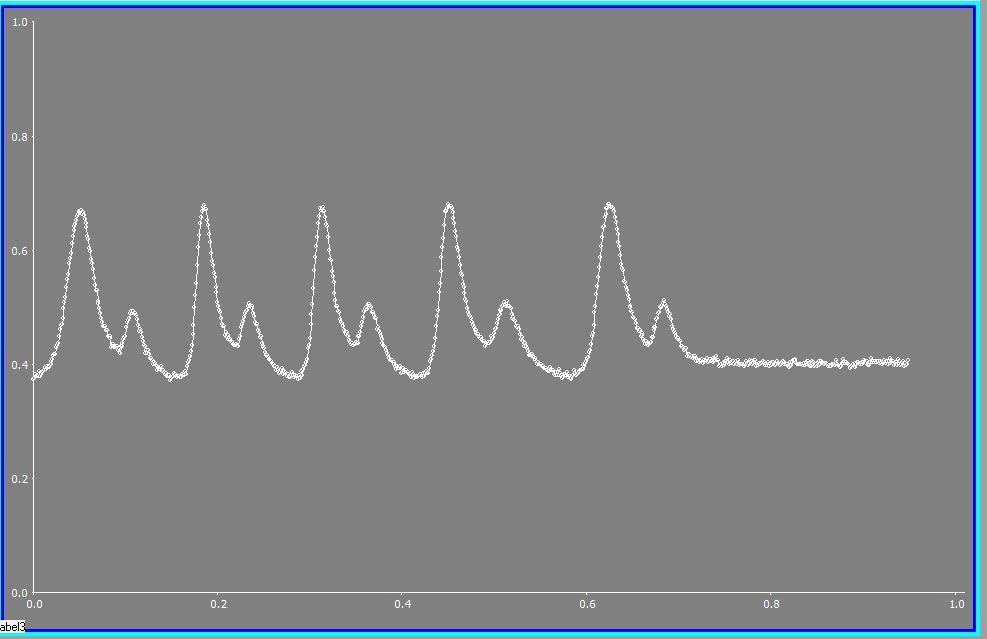
\includegraphics[height=0.3\textheight]{spectrum.JPG}
    \caption{Спектр зелёной линии таллия}
    \label{fig:spectr}
\end{figure}

По полученным данным определим величину сверхтонкого расщепления спектральной линии с длиной волны \(\lambda = 5350{,}46\,\text{\AA}\).

Сначала была выполнена замена параметра: построена интерферограмма \(I(P)\), представленная на рис.~\ref{fig:IP}. По графику были определены значения давления \(P_n\), соответствующие максимумам соседних порядков. Также наблюдались дополнительные максимумы меньшей интенсивности при давлении \(P_n'\). Полученные значения приведены в табл.~\ref{tab:1}.

\begin{table}[H]
\centering
\begin{tabular}{|c|c|c|c|c|c|}
\hline
\(n\) & 1 & 2 & 3 & 4 & 5 \\ \hline
\(P_n\), атм & 0.04 & 0.24 & 0.45 & 0.65 & 0.85 \\ \hline
\(P_n'\), атм & 0.12 & 0.32 & 0.52 & 0.73 & 0.91 \\ \hline
\end{tabular}
\caption{Значения давления, соответствующие максимумам соседних порядков и дополнительным максимумам}
\label{tab:1}
\end{table}

\begin{figure}[H]
    \centering
    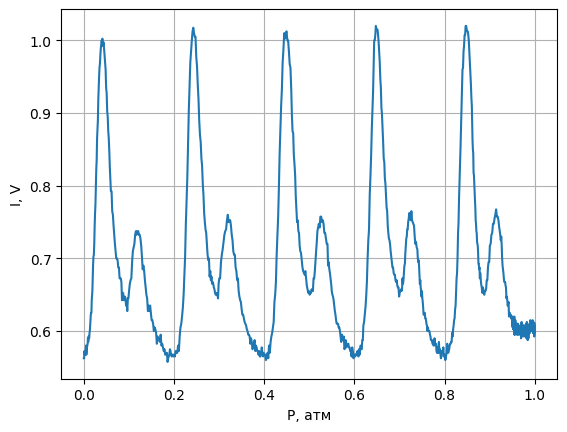
\includegraphics[height=0.4\textheight]{IP.png}
    \caption{Зависимость интенсивности \(I\) для зеленой линии таллия от давления \(P\) в барокамере}
    \label{fig:IP}
\end{figure}

По экспериментальным данным были вычислены:
среднее изменение давления, соответствующее изменению интерференционного порядка на единицу,
\(\Delta P = 0.20\,\text{атм}\),
и среднее смещение по давлению внутри одного порядка,
\(\Delta P' = 0.07\,\text{атм}\).

Из формул (11) и (12), приведённых в теоретической части, следует:
\begin{equation}
    \Delta m' = \frac{\Delta P'}{\Delta P},
\end{equation}
где \(\Delta m'\) — изменение интерференционного порядка, соответствующее сверхтонкому расщеплению спектральной линии.

Для полученных значений:
\begin{equation*}
    \Delta m' = 0.37.
\end{equation*}

Сверхтонкое расщепление определяется выражением
\begin{equation}
    \Delta \nu = \Delta m' \cdot \frac{1}{2d}.
\end{equation}

Подставляя экспериментальные данные, получаем:
\begin{equation*}
    \Delta \nu = 1.85\,\text{см}^{-1}.
\end{equation*}
    
    % Напиши здесь про давление и спектр и вставь графички. Обрати, пж, внимание, что формула (12) вроде как важная и используется
\end{itemize}


\section{Вывод}
В данной лабораторной работе была зарегистрирована сверхтонкая структура сперктральных линий с использованием спектрографа ИСП-51 и сканирующего интерферометра Фабри-Перо.
\end{document}
